\documentclass[12pt, titlepage]{article}

\usepackage{fullpage}
\usepackage[round]{natbib}
\usepackage{multirow}
\usepackage{booktabs}
\usepackage{tabularx}
\usepackage{graphicx}
\usepackage{float}
\usepackage{hyperref}
\usepackage{graphicx}
\usepackage{adjustbox}

\graphicspath{ {./images/} }
\hypersetup{
	colorlinks,
	citecolor=blue,
	filecolor=black,
	linkcolor=red,
	urlcolor=blue
}

\input{../../Comments}
\input{../../Common}

\newcounter{acnum}
\newcommand{\actheacnum}{AC\theacnum}
\newcommand{\acref}[1]{AC\ref{#1}}

\newcounter{ucnum}
\newcommand{\uctheucnum}{UC\theucnum}
\newcommand{\uref}[1]{UC\ref{#1}}

\newcounter{mnum}
\newcommand{\mthemnum}{M\themnum}
\newcommand{\mref}[1]{M\ref{#1}}

\begin{document}
	
	\title{System Design for \progname{}} 
	\author{\authname}
	\date{\today}
	
	\maketitle
	
	\pagenumbering{roman}
	
	\section{Revision History}
	
	\begin{tabularx}{\textwidth}{p{3cm}p{2cm}X}
		\toprule {\bf Date} & {\bf Version} & {\bf Notes}\\
		\midrule
		January 13 2023 & 1.0 & Initial Draft\\
		\bottomrule
	\end{tabularx}
	
	\newpage
	
	\section{Reference Material}
	
	This section records information for easy reference.
	
	\subsection{Abbreviations and Acronyms}
	
	\renewcommand{\arraystretch}{1.2}
	\begin{tabular}{l l} 
		\toprule		
		\textbf{symbol} & \textbf{description}\\
		\midrule 
		\progname & Explanation of program name\\
		\bottomrule
	\end{tabular}\\
	
	\newpage
	
	\tableofcontents
	
	\newpage
	
	\listoftables
	
	\listoffigures
	
	\newpage
	
	\pagenumbering{arabic}
	
	\section{Introduction}
	
	This document serves to illustrate and explain design decisions (in the context of alternatives) and the thought processes and considerations of the team that made said decisions.
	\section{Purpose}
	
	The purpose of this design documentation is to justify design decisions and prove that our final design meets all requirements as specified in the Software Requirements Specification (SRS).
	
	The purpose of this design documentation is to make clear current design choices, and to show why these designs were chosen over possible alternatives. This document also must prove that the current designs fulfill the requirements enumerated in the Software Requirements Specification (SRS) document.
	
	\section{Scope}
	
	\begin{figure}[H]
		\centering
		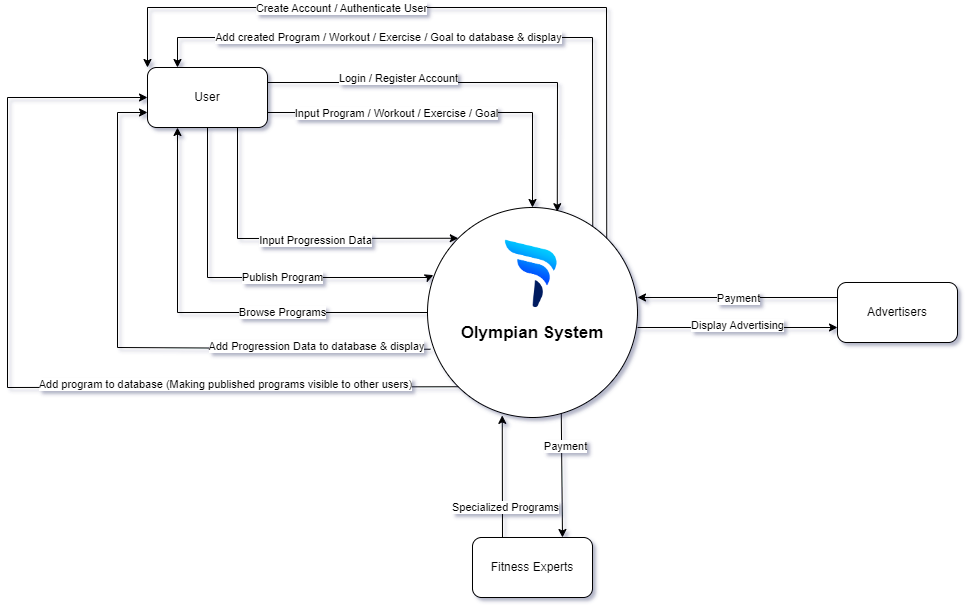
\includegraphics[scale=0.55]{system_context}
		\caption{System Context Diagram}
	\end{figure}

	\section{Project Overview}
	
	\subsection{Normal Behaviour}
  
	Normal behaviour for the application can be defined as the state of the available program when all FRs and NFRs are fulfilled. If an FR or NFR is not fulfilled, this is abnormal behaviour, and indicative of the occurrence of an undesired event.
	
	\subsection{Undesired Event Handling}
	
	An `undesired event' can comprise anything from incorrect user input to database failure to connectivity issues. 
	
	\textbf{Invalid User Input}: Whenever a user provides incorrect information to a form (e.g. an invalid email address during sign-up), an informative error message is displayed beneath the incorrectly filled field, and a visual queue is given in the form of highlighting the field in red to indicate error. To prevent annoying the user with error messages before they have actually made an error, forms will only display error messages after the first submit attempt. After an initial submit attempt, the error message will remain until the contents of the field are valid. This is to give the user information as to whether or not their entry is valid before having to submit again.
	
	\textbf{Connection/Database Failure}: If the application is unable to connect to the internet, and subsequently the server and database, an informative error message is displayed, informing the user to verify their internet connection. Note that a stretch goal for the future is to have the Olympian application save certain information locally to enable the user to perform certain functions offline. Changed local information would be synced with the database once connection is re-established. However, this is a stretch goal, and current requirements and designs list the database as the only information store, no data (other than an authentication token) is stored locally. If the database/server itself is failing, an appropriate message is displayed to the user. The message will indicate that the failure is not the fault of the user, but rather an internal failure outside of their control.
	\\
	
	Error messages are kept consistent and concise in format, to make errors easy for the user to recognize and act upon.
  
	\subsection{Component Diagram}

	\begin{figure}[H]
		\centering
		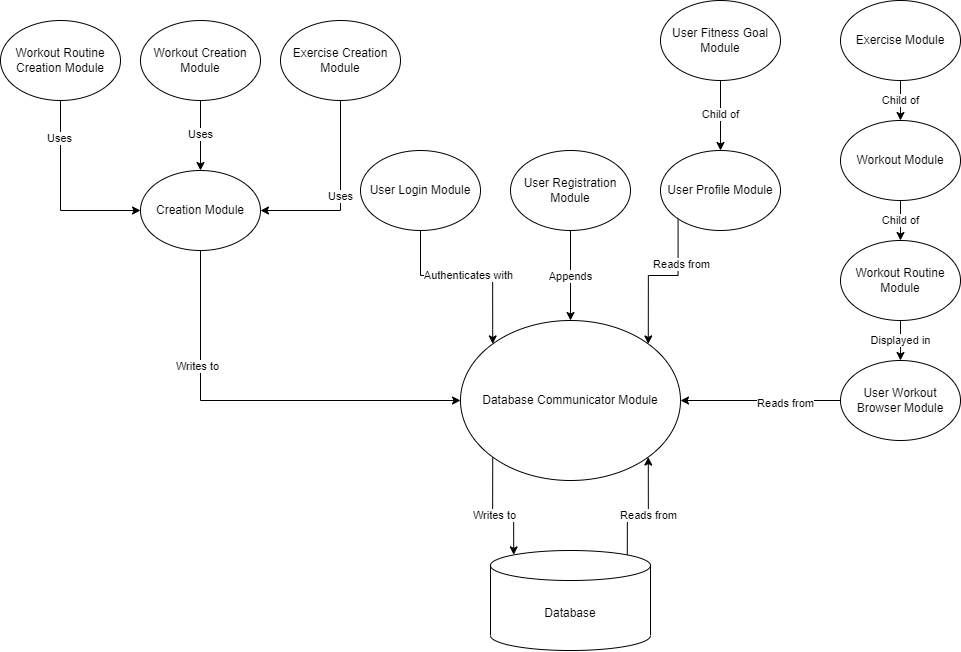
\includegraphics[width=\linewidth,keepaspectratio]{component_diagram}
    \caption{Diagram of Module Interactions}
	\end{figure}
	
	\subsection{Connection Between Requirements and Design} \label{SecConnection}
	
\begin{tabular}{ | m{20em} | m{20em} | }
		\hline
		Requirement & Design \\
		\hline
		The product shall appear minimal and straightforward & The application will contain an interface that only presents information that is necessary as to prevent cluttering and reduce minimality \\
		\hline
		The product shall use fonts of readable size to the target user group & Fonts of size 10-12 will be used across the application \\
		\hline
		The product shall be able to be used by untrained fitness enthusiasts and amateurs alike, who receive no training before using it & UI will be simplistic and consistent throughout, reducing the learning curve for users \\
		\hline
		The product shall be usable by users with hearing loss or partial blindness & The application will rely on both audio and visual cues to indicate correct inputs or application events \\
		\hline
		The application must inform users when maintenance is taking place and must warn them at least 1 day in advance & The application will utilize pop up screens to display important notifications to the user \\
		\hline
		The applicaiton will allow users to report offensive content and remove it from their feed & There will be a button on each post that gives user the option to report offensive content \\
		\hline

	\end{tabular}
	
	\section{System Variables}
	N/A
	
%	\subsection{Monitored Variables}
	
%	\subsection{Controlled Variables}
	
%	\subsection{Constants Variables}
	
	\section{User Interfaces}

  \begin{figure}[H]
		\centering
		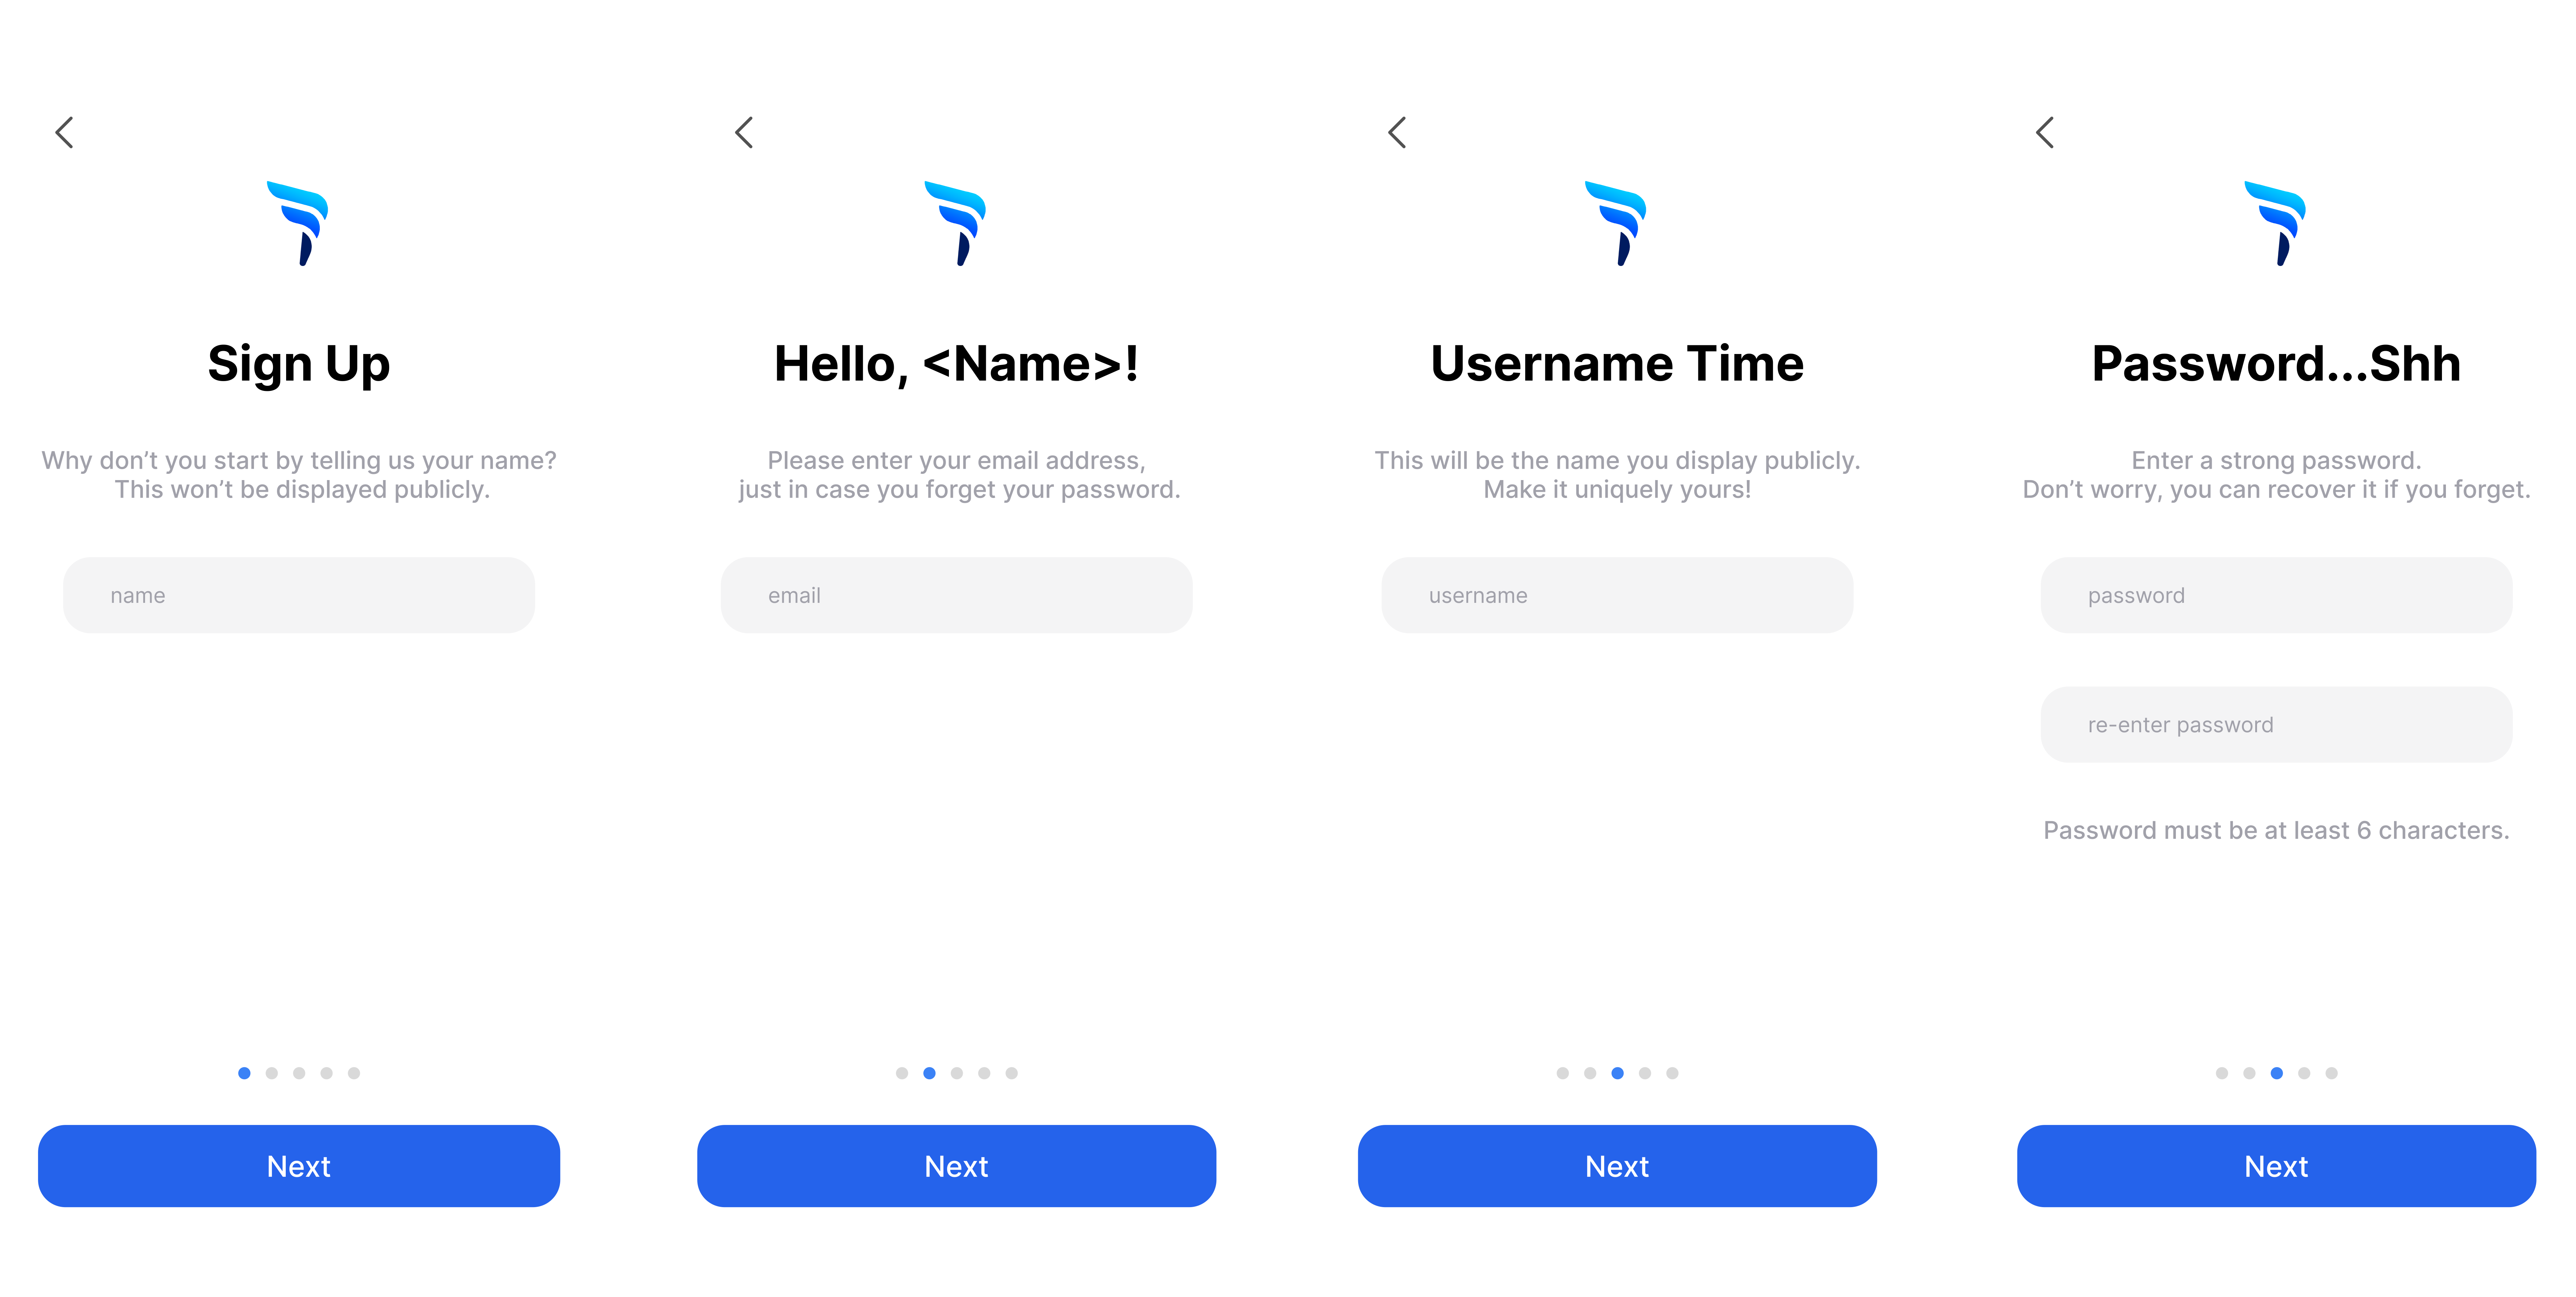
\includegraphics[width=\linewidth,keepaspectratio]{register_stack}
		\caption{Multi page register form}
	\end{figure}

  \begin{figure}[H]
		\centering
		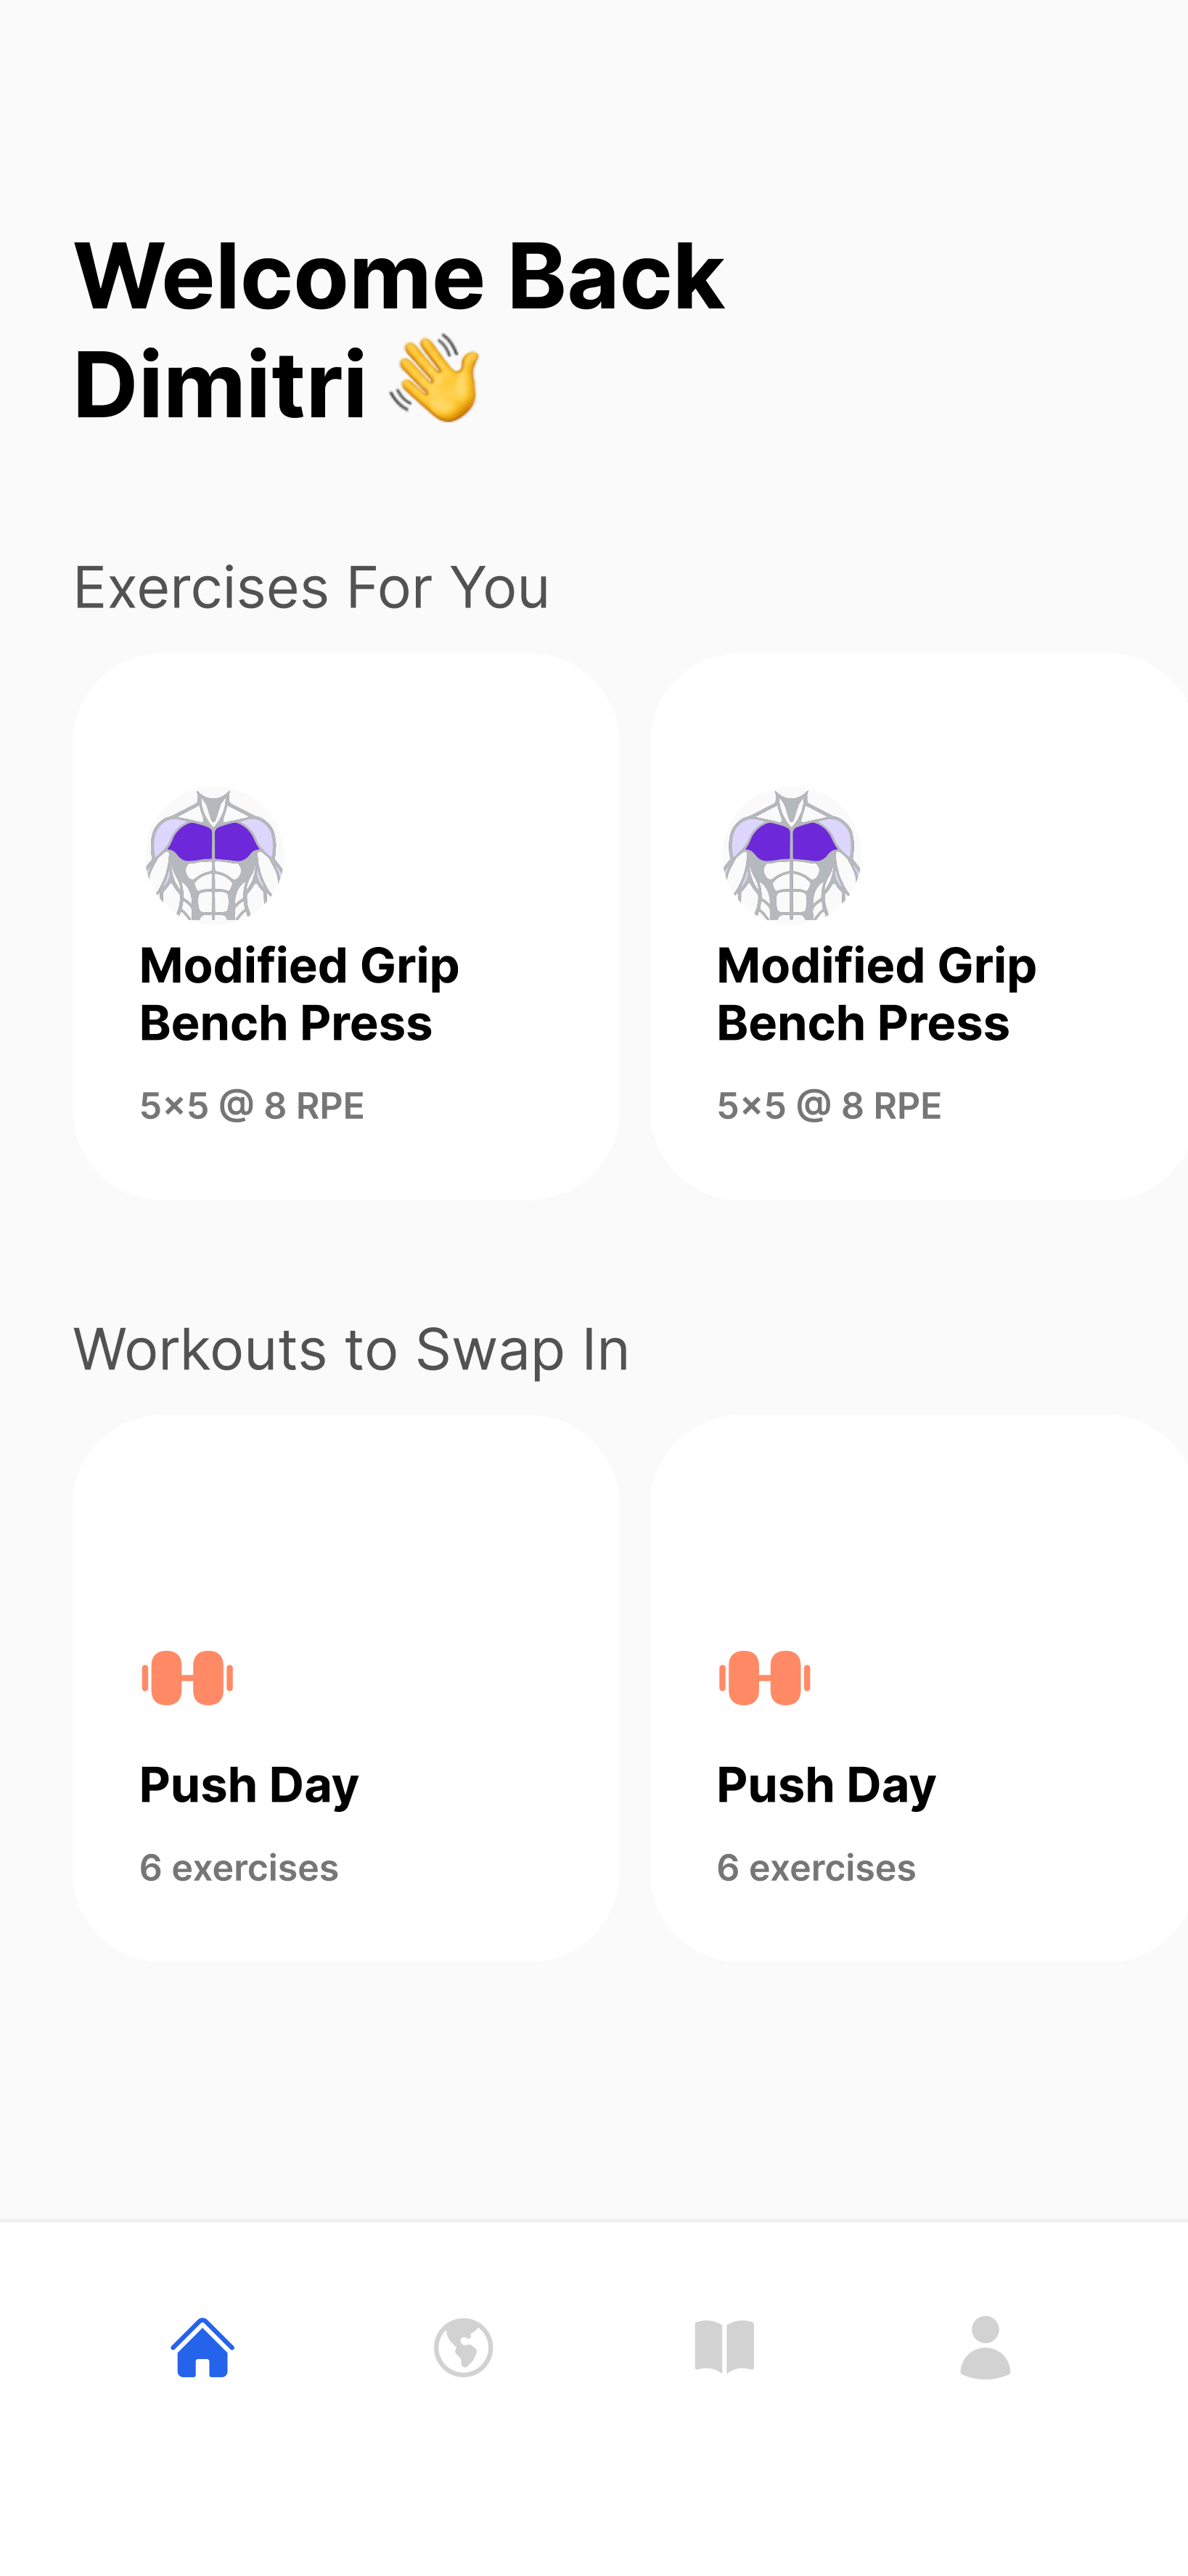
\includegraphics[scale=0.35]{home_screen}
		\caption{Home Screen (Landing page for logged in users)}
	\end{figure}

  \begin{figure}[H]
		\centering
		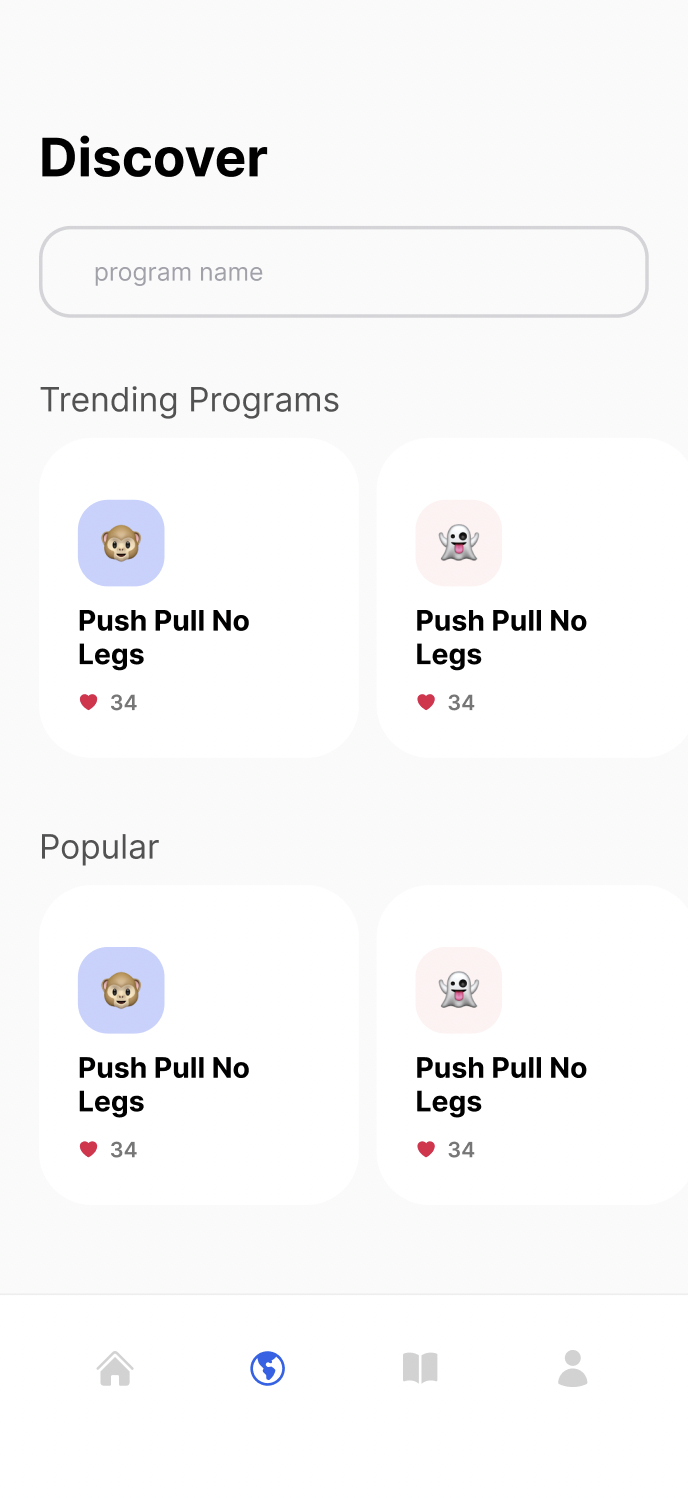
\includegraphics[scale=0.35]{discover_screen}
		\caption{Discover Screen}
	\end{figure}

  \begin{figure}[H]
		\centering
		\includegraphics[width=\linewidth,keepaspectratio]{static_program_stack}
    \caption{Static Program Stack: View when browsing programs from other authors or non active, personal programs.}
	\end{figure}

  \begin{figure}[H]
		\centering
		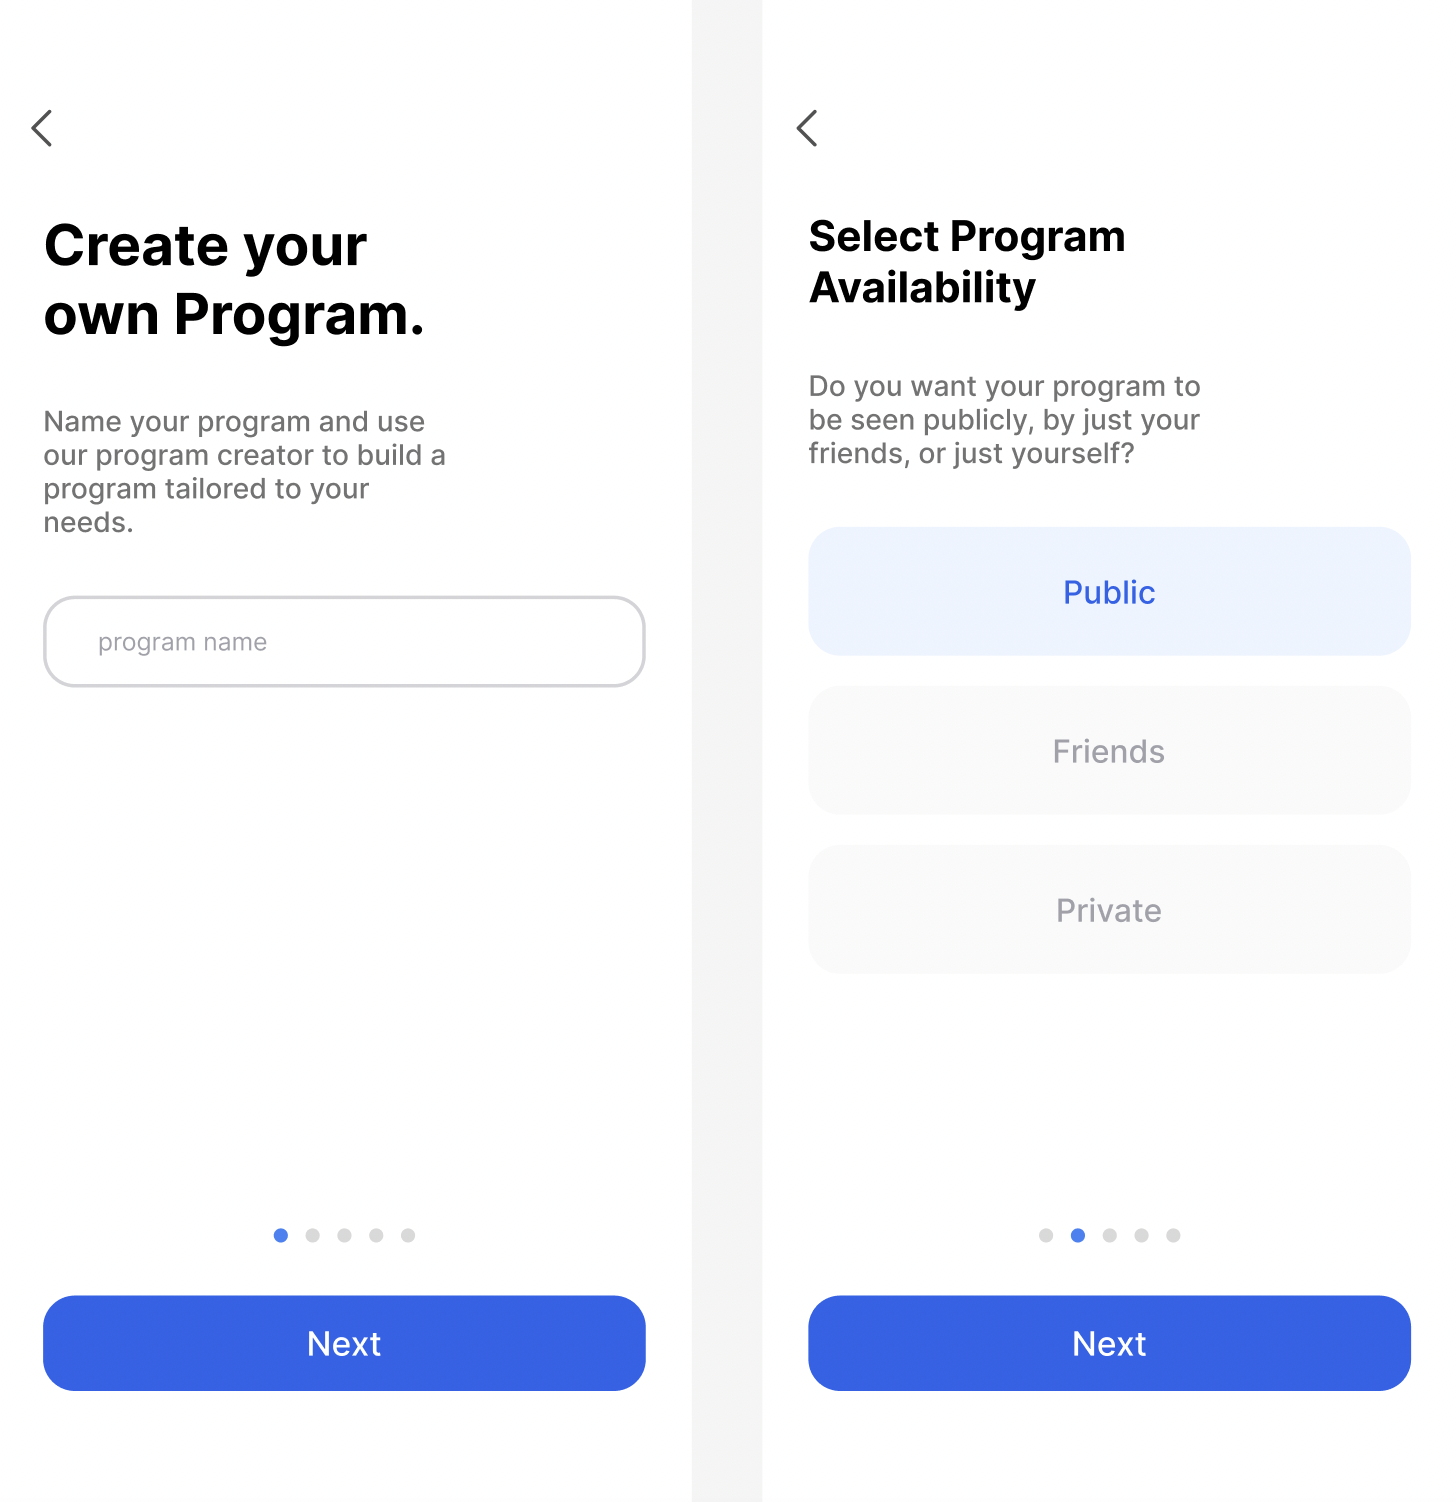
\includegraphics[width=\linewidth,keepaspectratio]{create_program_form}
    \caption{Multi page form for creating a program.}
	\end{figure}

  \begin{figure}[H]
		\centering
		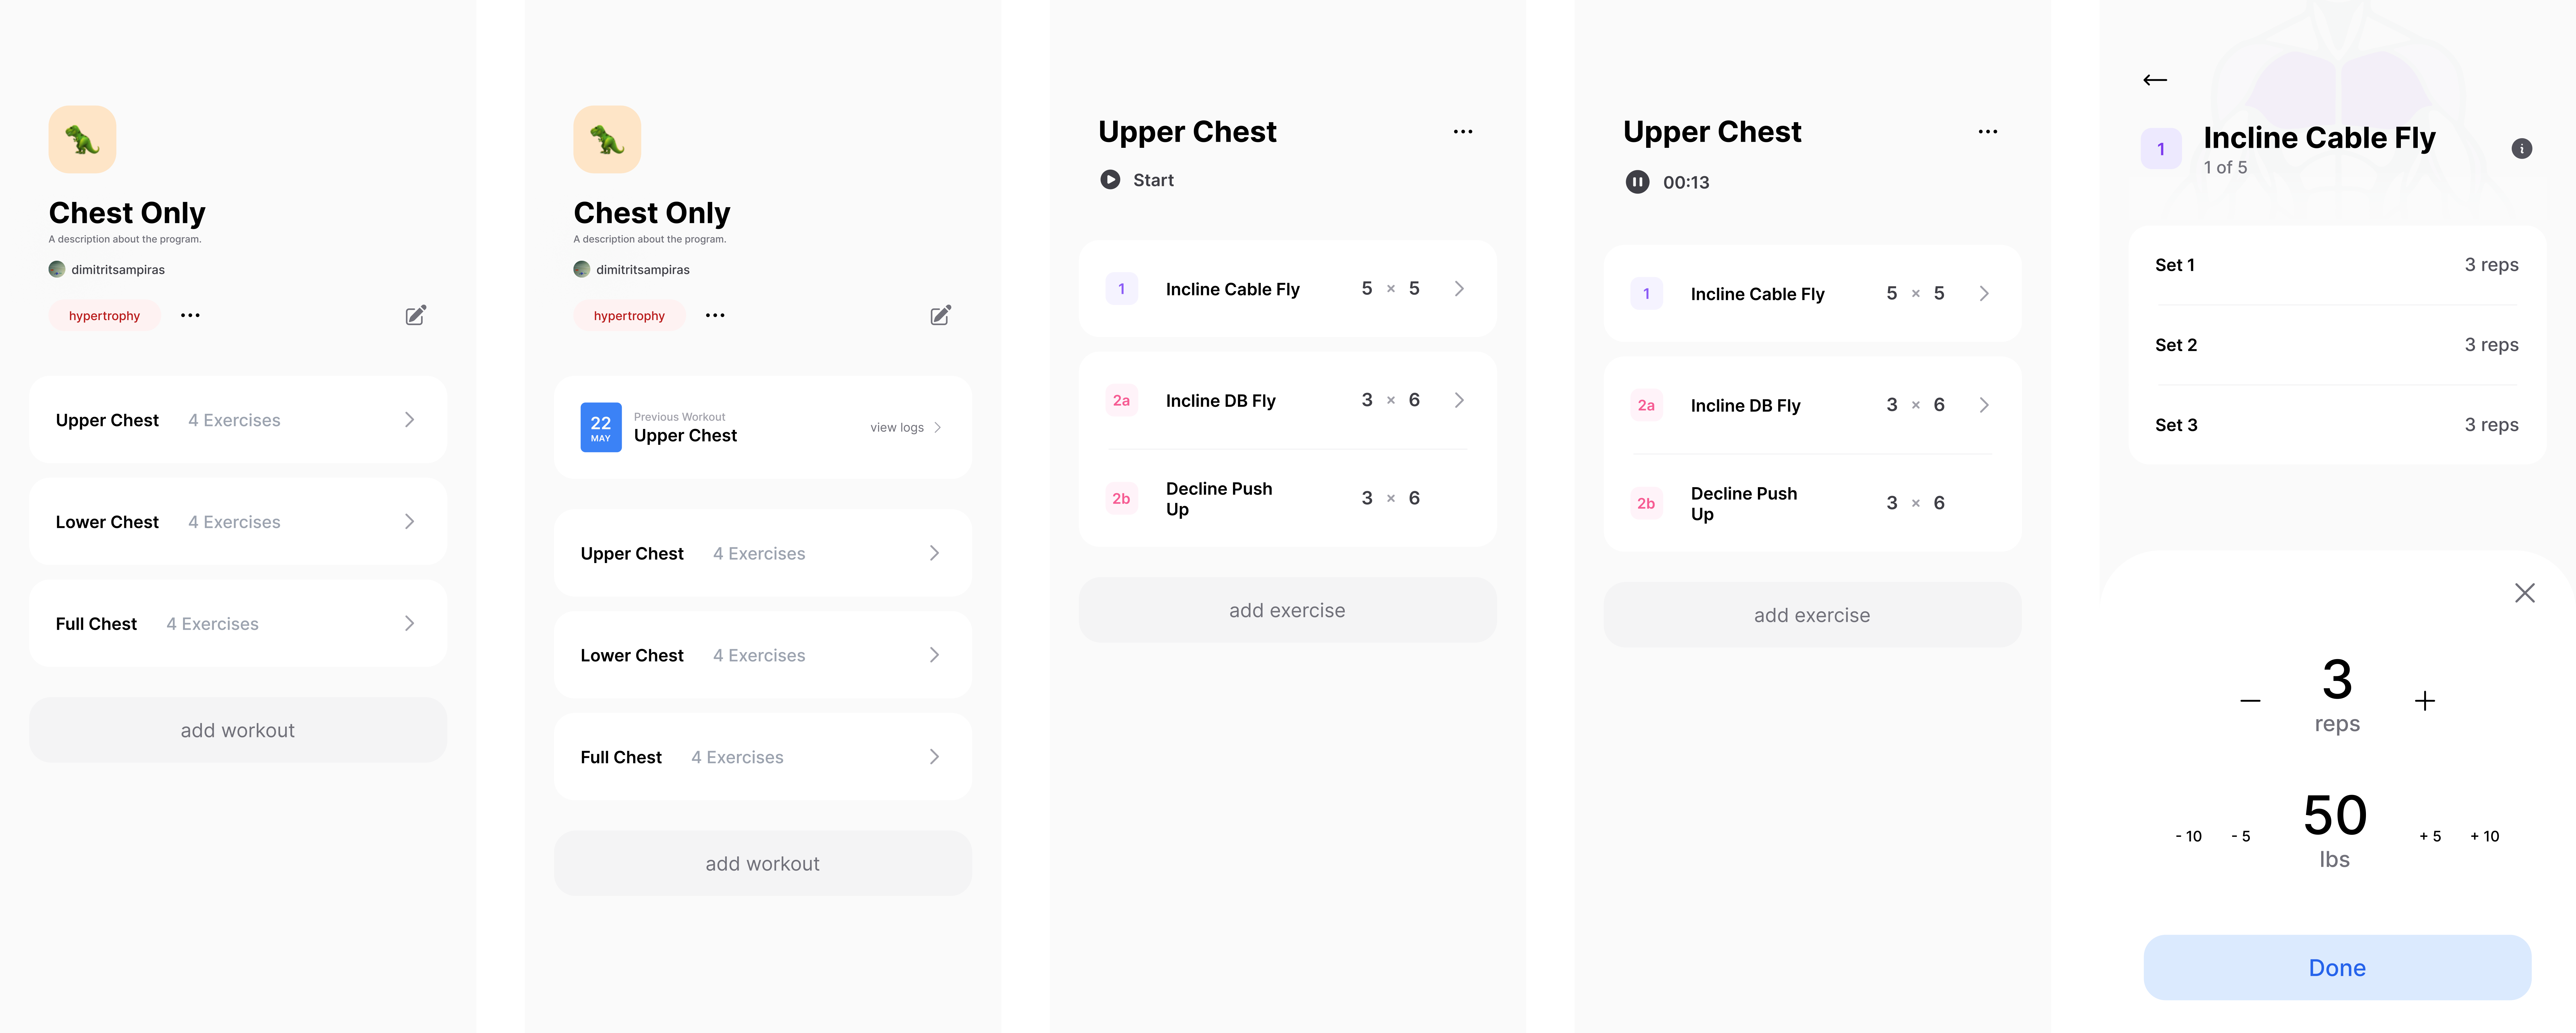
\includegraphics[width=\linewidth,keepaspectratio]{active_program_stack}
    \caption{Multi page form for creating a program.}
	\end{figure}
	
	\section{Design of Hardware}
	
	Olympian will run on mobile devices (e.g. iPhone, Samsung Galaxy) not designed or manufactured by the team.
	
	\section{Design of Electrical Components}
	
	N/A - See Section 9.
	
	\section{Design of Communication Protocols}
	
	Communication between client and server will be done with HTTP requests.

	There is no custom communication protocol used.
	
	\section{Timeline}

  Below is a timeline of the major milestones and the developers responsible for completing them.

  \begin{figure}[H]
		\centering
		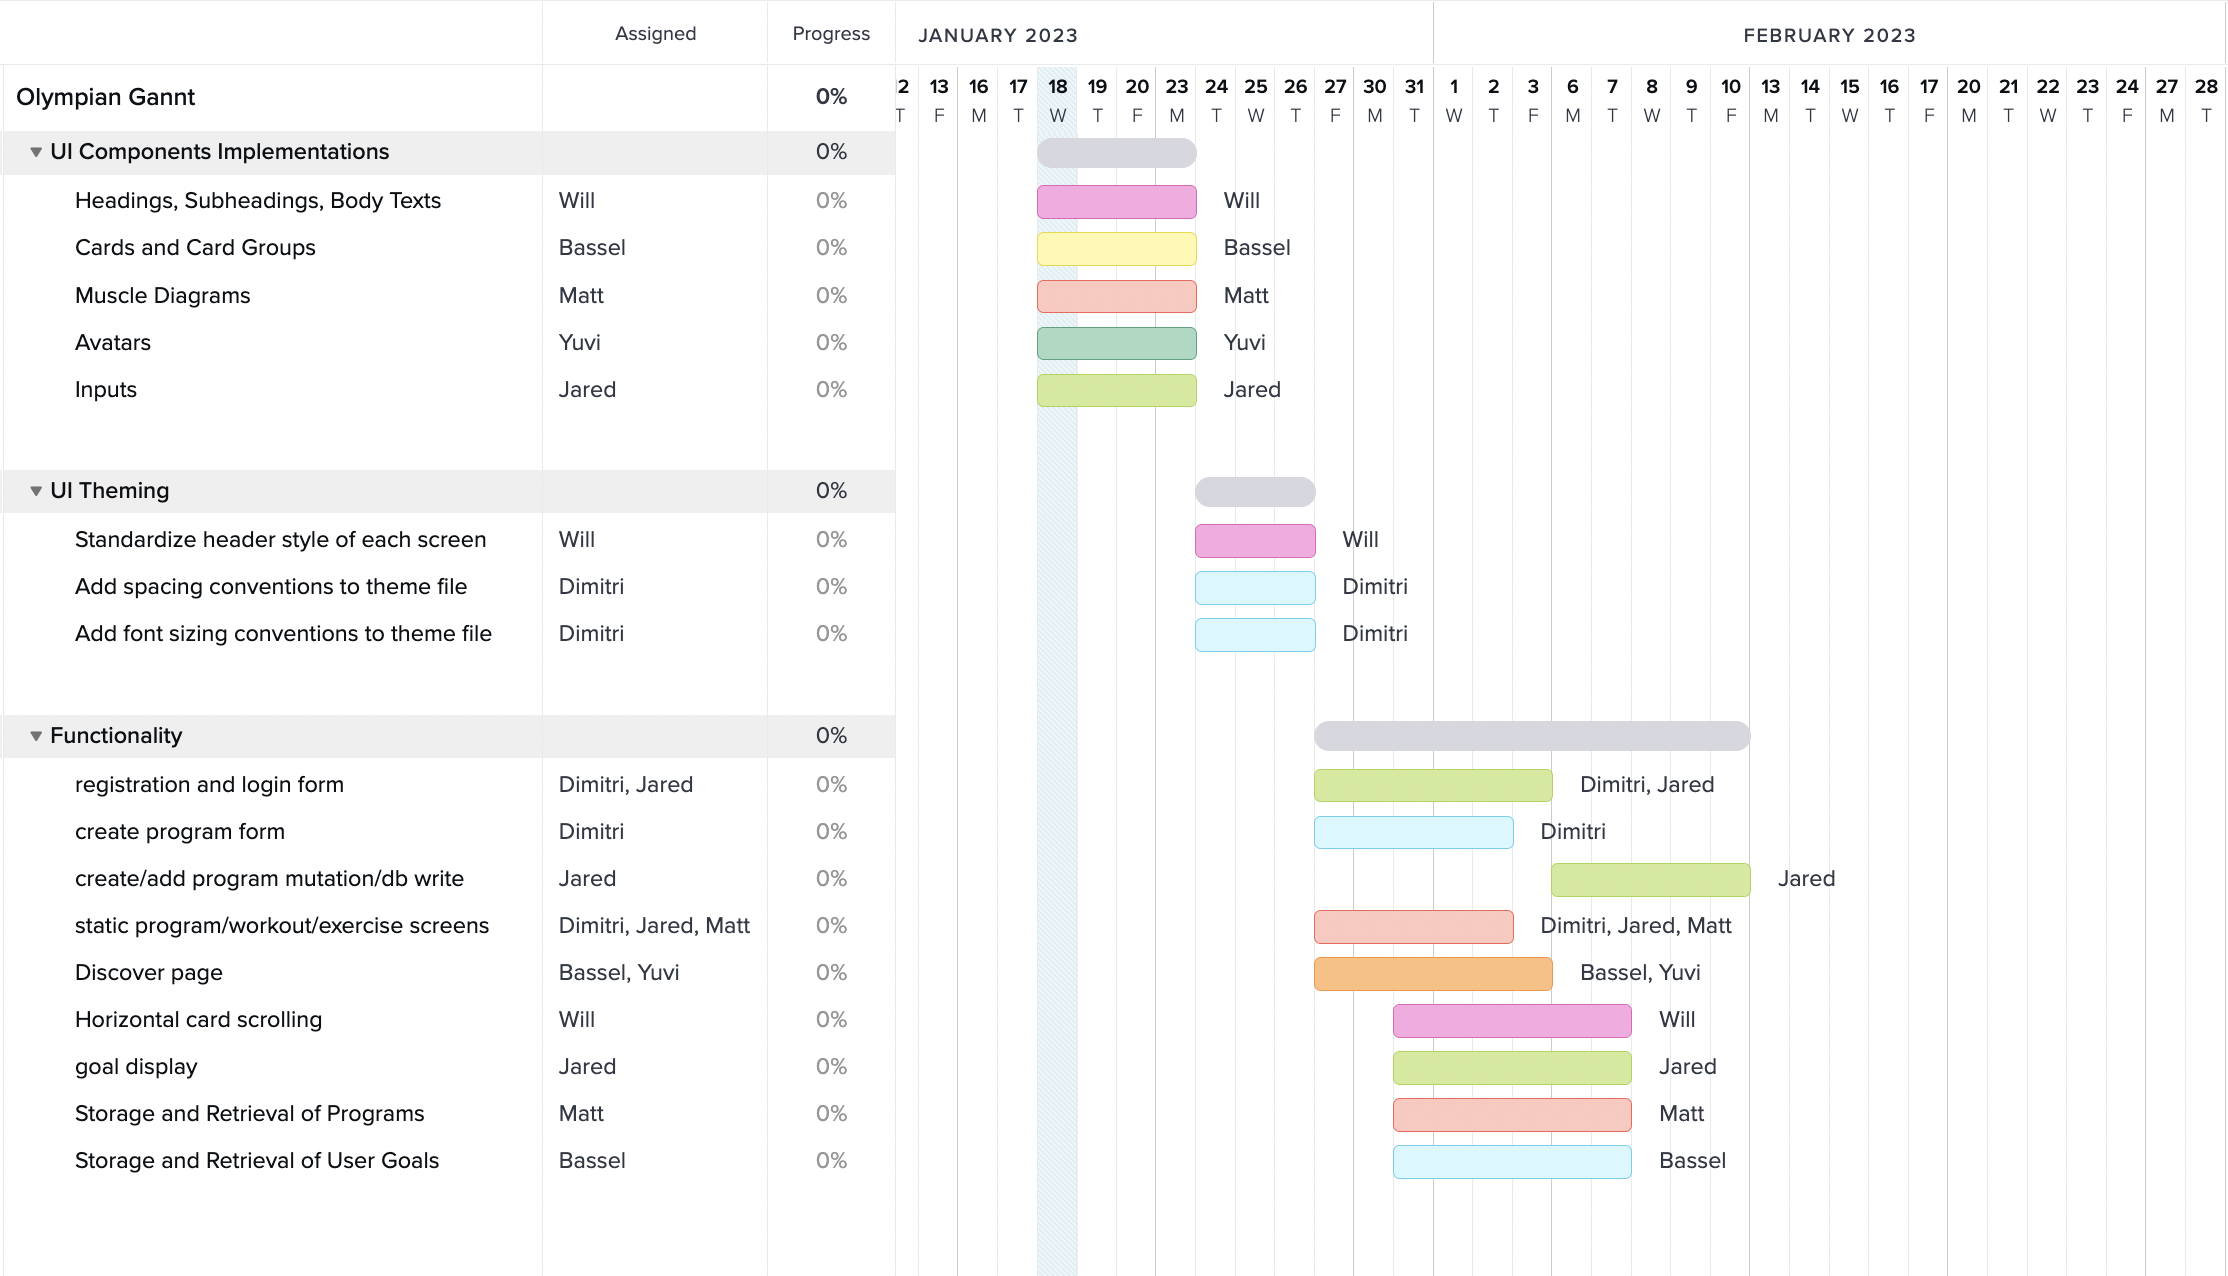
\includegraphics[width=\linewidth,keepaspectratio]{gantt_chart}
    \caption{Multi page form for creating a program.}
	\end{figure}
	
	
	% \bibliographystyle {plainnat}
	% \bibliography{../../../refs/References}
	
	\newpage{}
	
	\appendix
	
	\section{Interface}
	
	See Figma.
	
	\section{Mechanical Hardware}
	N/A
	
	\section{Electrical Components}
	N/A
	
	\section{Communication Protocols}
	The project employs Hyper Text Transfer Protocol (HTTP), enabling the client to communicate with the server and database through HTTP requests.
	
	\section{Reflection}
	
	The information in this section will be used to evaluate the team members on the
	graduate attribute of Problem Analysis and Design.  Please answer the following questions:
	
	\begin{enumerate}
		\item What are the limitations of your solution?  Put another way, given
		unlimited resources, what could you do to make the project better? (LO\_ProbSolutions)
		\item Give a brief overview of other design solutions you considered.  What
		are the benefits and tradeoffs of those other designs compared with the chosen
		design?  From all the potential options, why did you select documented design?
		(LO\_Explores)
	\end{enumerate}
	
\end{document}
